\documentclass[aspectratio=169,14pt]{beamer}
\usetheme{default}
\usepackage{fontspec}
\setmainfont{texgyrepagella-regular.otf}[BoldFont=texgyrepagella-bold.otf,ItalicFont=texgyrepagella-italic.otf,BoldItalicFont=texgyrepagella-bolditalic.otf]
\setsansfont{texgyreheros-regular.otf}[BoldFont=texgyreheros-bold.otf,ItalicFont=texgyreheros-italic.otf,BoldItalicFont=texgyreheros-bold.otf,BoldItalicFeatures={FakeSlant=0.2}]
\setmonofont{lmmono10-regular.otf}[Scale=0.85]
\setbeamertemplate{navigation symbols}{}
\usepackage{pgfpages}
\newif\ifpresenter
\ifdefined\PresenterVersion\presentertrue\else\presenterfalse\fi
\ifpresenter
  \setbeameroption{show notes on second screen=right}
  \setbeamertemplate{note page}[plain]
\fi
\usepackage{amsmath,amssymb,bm,booktabs,array,graphicx,xcolor}
\usepackage{tikz,pgfplots,adjustbox,listings,xurl}
\pgfplotsset{compat=1.18}
\usetikzlibrary{arrows.meta,positioning,calc,fit,shapes.geometric,decorations.pathreplacing,patterns}
% UIUC official brand colors, verified 2026-10-23.
% https://brand.illinois.edu/visual-identity/color
\definecolor{IlliniOrange}{HTML}{FF5F05}
\definecolor{IlliniBlue}{HTML}{13294B}
\definecolor{Storm}{HTML}{707372}
\definecolor{LightStorm}{HTML}{C6C7C6}
\definecolor{Industrial}{HTML}{1D58A7}
\definecolor{Patina}{HTML}{007E8E}
\tikzset{>=Stealth, every node/.style={font=\small,text=IlliniBlue}, box/.style={draw=IlliniBlue,rounded corners=2pt,align=center,inner sep=6pt,execute at begin node=\hyphenpenalty10000\relax}, orangebox/.style={box,draw=IlliniOrange,very thick}, edge/.style={->,thick,IlliniBlue}, accent/.style={->,very thick,IlliniOrange}}
\pgfplotsset{every axis/.append style={width=13.5cm,height=6.5cm,axis line style={IlliniBlue},tick label style={font=\small,text=IlliniBlue},label style={font=\small,text=IlliniBlue},legend style={font=\small,draw=none,fill=white},grid style={LightStorm},major grid style={LightStorm},axis lines=left,clip=false}, every axis plot/.append style={thick}}

\definecolor{slidepaper}{RGB}{234,220,201}
\setbeamercolor{background canvas}{bg=slidepaper}
\setbeamercolor{normal text}{fg=IlliniBlue}
\setbeamercolor{frametitle}{fg=IlliniBlue}
\setbeamercolor{title}{fg=IlliniBlue}
\setbeamercolor{item}{fg=IlliniOrange}
\setbeamerfont{frametitle}{size=\large,series=\bfseries}
\setbeamerfont{title}{size=\Large,series=\bfseries}
\setbeamertemplate{itemize item}{\color{IlliniOrange}$\bullet$}
\setbeamertemplate{itemize subitem}{\color{IlliniOrange}\footnotesize$\circ$}
\setbeamercolor{orangerule}{bg=IlliniOrange}
\setbeamertemplate{headline}{\begin{beamercolorbox}[wd=\paperwidth,ht=0.1cm,dp=0.1cm]{orangerule}\end{beamercolorbox}}
\setbeamertemplate{footline}{\begin{beamercolorbox}[wd=\paperwidth,ht=0.1cm,dp=0.1cm]{orangerule}\end{beamercolorbox}}
\setbeamersize{text margin left=0.65cm,text margin right=0.65cm}
\setlength{\leftmargini}{1.1em}
\newenvironment{slidebullets}{\begin{itemize}\setlength\itemsep{0.8em}}{\end{itemize}}
\pgfplotsset{every axis/.append style={legend style={fill=slidepaper}}}
\lstdefinelanguage{CoursePython}{keywords={from,import,for,in,if,else,def,return,assert,True,False,None},sensitive=true,morecomment=[l]{\#},morestring=[b]',morestring=[b]"}
\lstset{language=CoursePython,basicstyle=\ttfamily\small,keywordstyle=\color{IlliniBlue}\bfseries,commentstyle=\color{Storm},stringstyle=\color{IlliniBlue},showstringspaces=false,breaklines=true,columns=fullflexible,keepspaces=true,frame=none,aboveskip=0.7em,belowskip=0.7em}
\newcommand{\E}{\mathbb E}
\newcommand{\Var}{\operatorname{Var}}
\newcommand{\Cov}{\operatorname{Cov}}
\hypersetup{colorlinks=true,urlcolor=IlliniBlue,linkcolor=IlliniBlue}

\title{Marketing Analytics}
\subtitle{Causal Comparisons and Policy Evaluation}
\author{By Nathan Yang}
\date{Session 10}
\begin{document}
\begin{frame}
\titlepage
\end{frame}
\begin{frame}{A Repair-Policy Question}
\usebeamercolor[fg]{normal text}
\vfill
\begin{slidebullets}
\item A policy may change the cost of restoring restaurant availability.
\item A national before-after change also includes common shocks.
\item The target is the change attributable to the policy over a defined horizon.
\end{slidebullets}
\vfill
\note{The McBroken setting motivates a causal question. The supplied panel does not by itself establish a valid untreated comparison for a policy affecting the same environment broadly.

M6, Section 6.16, Marketing Analytics Lecture Notes. \url{../06_Lecture_Notes/modules/M06_Causal_Inference_and_Experiments.md}}
\end{frame}
\begin{frame}{Difference-in-Differences}
\usebeamercolor[fg]{normal text}
\noindent Subtract the comparison group's change from the treated group's change.
\medskip
\[
\widehat\tau=(\bar Y_{T,post}-\bar Y_{T,pre})-(\bar Y_{C,post}-\bar Y_{C,pre})
\]
\medskip
\noindent Parallel untreated trends connect the observed changes to a causal effect.
\note{Different starting levels can be compatible with the design. The assumption concerns untreated changes, not identical outcome levels.

M6, Section 6.8, Marketing Analytics Lecture Notes. \url{../06_Lecture_Notes/modules/M06_Causal_Inference_and_Experiments.md}}
\end{frame}
\begin{frame}{The Counterfactual Trend}
\usebeamercolor[fg]{normal text}
\centering
\begingroup
\begin{adjustbox}{max width=0.98\textwidth,max totalheight=0.65\textheight}
% Original synthetic teaching figure; see corresponding module.
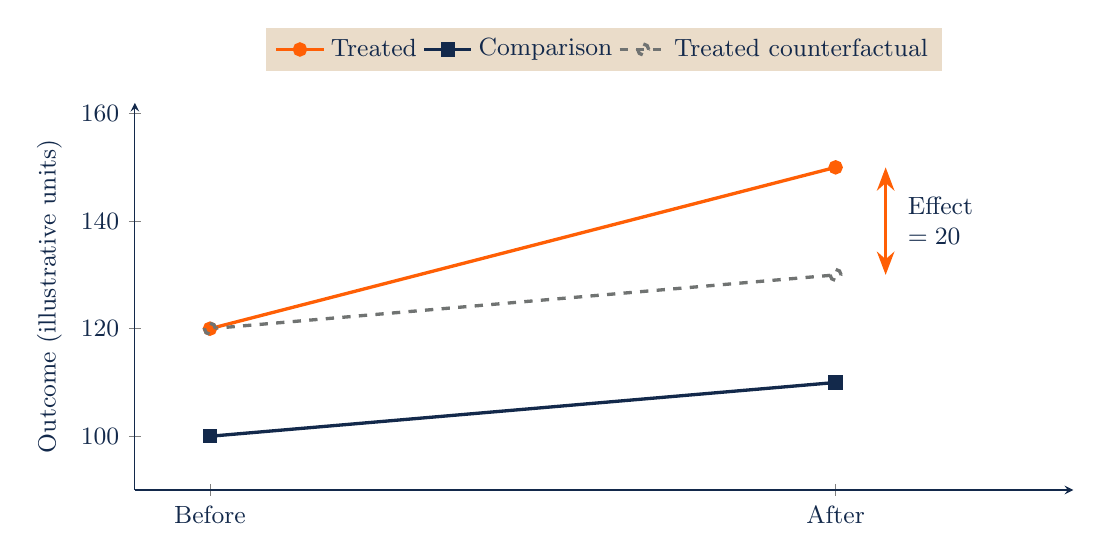
\begin{tikzpicture}
\begin{axis}[xmin=-.12,xmax=1.38,ymin=90,ymax=162,xtick={0,1},xticklabels={Before,After},ylabel={Outcome (illustrative units)},legend style={at={(.5,1.08)},anchor=south,legend columns=3}]
\addplot[IlliniOrange,mark=*,very thick] coordinates {(0,120)(1,150)};
\addplot[IlliniBlue,mark=square*,very thick] coordinates {(0,100)(1,110)};
\addplot[Storm,dashed,mark=o,very thick] coordinates {(0,120)(1,130)};
\legend{Treated,Comparison,Treated counterfactual}
\draw[<->,IlliniOrange,very thick] (axis cs:1.08,130)--(axis cs:1.08,150);
\node[anchor=west,align=left] at (axis cs:1.1,140) {Effect\\$=20$};
\end{axis}
\end{tikzpicture}

\end{adjustbox}
\endgroup
\par\medskip
{\small Synthetic outcomes. Treated sales rise 120 to 150 and comparison sales 100 to 110.\par}
\note{The dashed path is an implied counterfactual. A treatment-specific demand shock at the same time would challenge the interpretation.

M6, Section 6.8, Marketing Analytics Lecture Notes. \url{../06_Lecture_Notes/modules/M06_Causal_Inference_and_Experiments.md}}
\end{frame}
\begin{frame}{Design Checks}
\usebeamercolor[fg]{normal text}
\vfill
\begin{slidebullets}
\item Examine pre-treatment outcomes and institutional timing.
\item Consider anticipation, spillovers, and changing composition.
\item Match the comparison group to the policy's untreated counterfactual.
\end{slidebullets}
\vfill
\note{A nonsignificant pre-trend test does not establish parallel trends. With staggered adoption and heterogeneous effects, the choice of comparison groups and aggregation becomes especially important.

M6, Section 6.8, Marketing Analytics Lecture Notes. \url{../06_Lecture_Notes/modules/M06_Causal_Inference_and_Experiments.md}}
\end{frame}
\begin{frame}{McBroken and the Comparison Group}
\usebeamercolor[fg]{normal text}
\centering
\begingroup
\begin{adjustbox}{max width=0.98\textwidth,max totalheight=0.65\textheight}
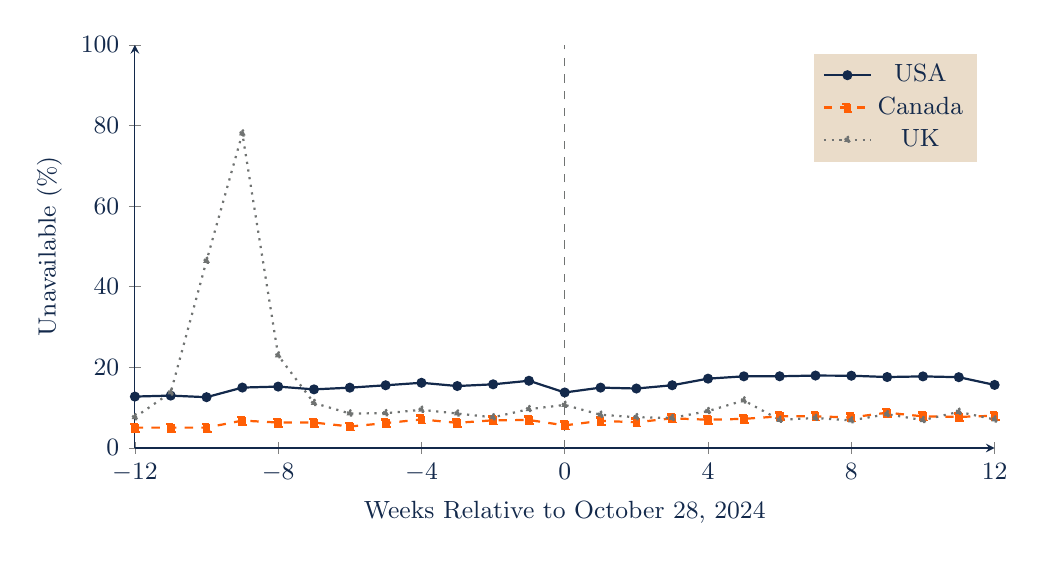
\begin{tikzpicture}
\begin{axis}[width=12.5cm,height=6.7cm,xmin=-12,xmax=12,ymin=0,ymax=100,
 xlabel={Weeks Relative to October 28, 2024},ylabel={Unavailable (\%)},
 xtick={-12,-8,-4,0,4,8,12},legend style={at={(0.98,0.98)},anchor=north east}]
\addplot[IlliniBlue,mark=*,mark size=1.4pt] coordinates {(-12,12.749681) (-11,12.987561) (-10,12.593262) (-9,14.981949) (-8,15.221368) (-7,14.533786) (-6,14.955595) (-5,15.550071) (-4,16.168717) (-3,15.363128) (-2,15.787402) (-1,16.672954) (0,13.764451) (1,14.967462) (2,14.744526) (3,15.556331) (4,17.195675) (5,17.769038) (6,17.781690) (7,17.960320) (8,17.923536) (9,17.594193) (10,17.753121) (11,17.558651) (12,15.641664)};
\addplot[IlliniOrange,dashed,mark=square*,mark size=1.4pt] coordinates {(-12,5.042017) (-11,5.042017) (-10,5.042017) (-9,6.792717) (-8,6.302521) (-7,6.302521) (-6,5.322129) (-5,6.162465) (-4,7.072829) (-3,6.232493) (-2,6.862745) (-1,6.932773) (0,5.602241) (1,6.722689) (2,6.372549) (3,7.352941) (4,7.002801) (5,7.212885) (6,7.843137) (7,7.843137) (8,7.563025) (9,8.753501) (10,7.843137) (11,7.703081) (12,7.983193)};
\addplot[Storm,dotted,mark=triangle*,mark size=1.4pt] coordinates {(-12,7.614608) (-11,13.752914) (-10,46.428571) (-9,78.027950) (-8,22.950820) (-7,11.145752) (-6,8.547009) (-5,8.618012) (-4,9.464701) (-3,8.533747) (-2,7.602793) (-1,9.619860) (0,10.678098) (1,8.229814) (2,7.626459) (3,7.447634) (4,9.147287) (5,11.782946) (6,6.976744) (7,7.441860) (8,6.832298) (9,8.372093) (10,6.904577) (11,8.963367) (12,7.054264)};
\legend{USA,Canada,UK}
\draw[Storm,dashed] (axis cs:0,0)--(axis cs:0,100);
\end{axis}
\end{tikzpicture}

\end{adjustbox}
\endgroup
\par\medskip
{\small A policy-analysis design requires a credible untreated comparison.\par}
\note{The course case retains missing dates and unknown statuses. Those measurement issues should be addressed before interpreting an apparent policy break.

M6, Section 6.16, Marketing Analytics Lecture Notes. \url{../06_Lecture_Notes/modules/M06_Causal_Inference_and_Experiments.md}}
\end{frame}
\begin{frame}{Regression Discontinuity}
\usebeamercolor[fg]{normal text}
\vfill
\begin{slidebullets}
\item Eligibility can change at a known score threshold.
\item Nearby units require continuity of other outcome determinants.
\item The resulting effect is local to the cutoff and compliance behavior.
\end{slidebullets}
\vfill
\note{Manipulation of the score and discontinuities in other policies threaten the comparison. Bandwidth and functional form should be assessed within the design.

M6, Section 6.9, Marketing Analytics Lecture Notes. \url{../06_Lecture_Notes/modules/M06_Causal_Inference_and_Experiments.md}}
\end{frame}
\begin{frame}{Instrumental Variables}
\usebeamercolor[fg]{normal text}
\vfill
\begin{slidebullets}
\item The instrument shifts treatment or price.
\item Exclusion restricts its other paths to the outcome.
\item Relevance alone does not establish exclusion.
\end{slidebullets}
\vfill
\note{Under the appropriate binary-treatment conditions, IV can identify a local effect for compliers. The interpretation depends on the assignment mechanism and monotonicity, as well as the first stage.

M6, Section 6.9, Marketing Analytics Lecture Notes. \url{../06_Lecture_Notes/modules/M06_Causal_Inference_and_Experiments.md}}
\end{frame}
\begin{frame}{Recommendation Logs Select Exposure}
\usebeamercolor[fg]{normal text}
\vfill
\begin{slidebullets}
\item Frequent buyers may usually see product A.
\item Occasional buyers may usually see product B.
\item Their raw click rates compare different customer populations.
\end{slidebullets}
\vfill
\note{A logged outcome is observed after a selected display. A policy comparison must account for the distribution of customers and actions that generated those observations.

M6, Section 6.7.1, Marketing Analytics Lecture Notes. \url{../06_Lecture_Notes/modules/M06_Causal_Inference_and_Experiments.md}}
\end{frame}
\begin{frame}{Exposure Adjustment Reverses the Ranking}
\usebeamercolor[fg]{normal text}
\centering
\begingroup
\begin{adjustbox}{max width=0.98\textwidth,max totalheight=0.65\textheight}
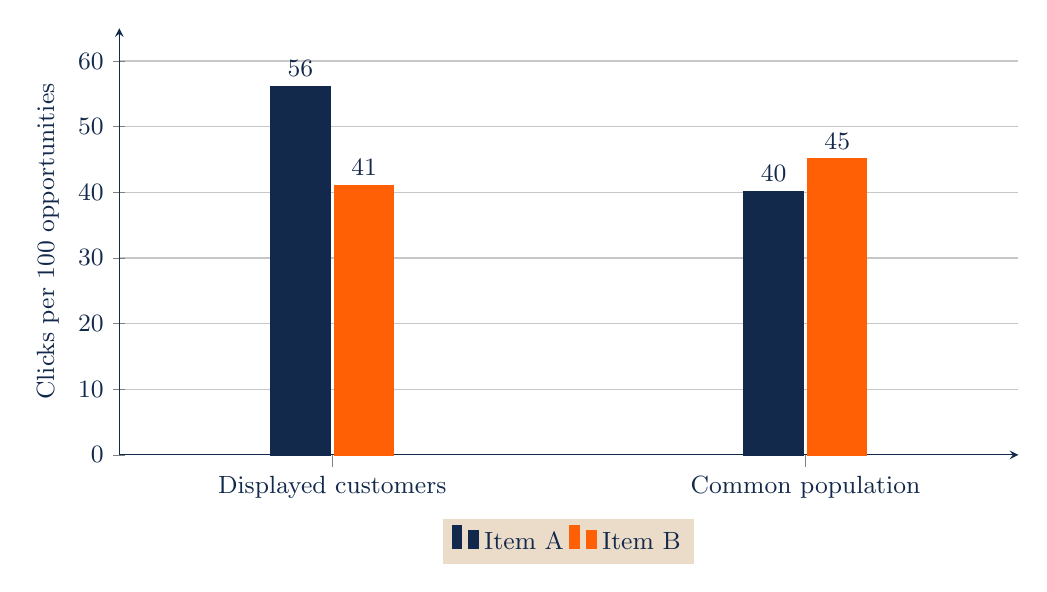
\begin{tikzpicture}
\begin{axis}[ybar,bar width=21pt,width=13cm,height=7cm,
  symbolic x coords={Displayed customers,Common population},
  xtick=data,ymin=0,ymax=65,ytick={0,10,20,30,40,50,60},
  ylabel={Clicks per 100 opportunities},
  enlarge x limits=.45,ymajorgrids=true,
  nodes near coords,point meta=y,
  every node near coord/.append style={font=\small},
  legend style={at={(.5,-.15)},anchor=north,legend columns=2}]
\addplot[fill=IlliniBlue,draw=IlliniBlue] coordinates
  {(Displayed customers,56) (Common population,40)};
\addplot[fill=IlliniOrange,draw=IlliniOrange] coordinates
  {(Displayed customers,41) (Common population,45)};
\legend{Item A,Item B}
\end{axis}
\end{tikzpicture}

\end{adjustbox}
\endgroup
\par\medskip
{\small Synthetic randomized logging within frequent and occasional buyer groups.\par}
\note{The constructed logging design gives A probability 0.90 for frequent buyers and 0.10 for occasional buyers. B receives the complement. The common-population comparison holds customer mix fixed.

M6, Section 6.7.2, Marketing Analytics Lecture Notes. \url{../06_Lecture_Notes/modules/M06_Causal_Inference_and_Experiments.md}}
\end{frame}
\begin{frame}{Inverse-Propensity Policy Value}
\usebeamercolor[fg]{normal text}
\noindent Weight each observed outcome by target-policy probability over logging probability.
\medskip
\[
\widehat V(\pi)=\frac{1}{n}\sum_i\frac{\pi(A_i\mid X_i)}{p_0(A_i\mid X_i)}Y_i
\]
\medskip
\noindent The denominator counts every eligible logged opportunity.
\note{Identification requires the relevant exchangeability condition and positive logging support wherever the target policy acts. A randomized logging policy can supply known assignment probabilities.

M6, Section 6.7.1, Marketing Analytics Lecture Notes. \url{../06_Lecture_Notes/modules/M06_Causal_Inference_and_Experiments.md}}
\end{frame}
\begin{frame}[fragile]{A Common-Population Calculation}
\usebeamercolor[fg]{normal text}
\noindent Synthetic clicks and logging probabilities identify the two policy values.
\begin{lstlisting}
n = 1000
value_a = (270 / 0.90 + 10 / 0.10) / n
value_b = (25 / 0.10 + 180 / 0.90) / n
raw_a = 280 / 500
raw_b = 205 / 500
assert (value_a, value_b) == (0.40, 0.45)
\end{lstlisting}
{\small The raw ranking and policy-value ranking disagree.\par}
\note{An independent check averages the two group-specific response rates under equal population weights. The small-probability cells receive large weights and contribute substantial uncertainty.

M6, Section 6.7.2, Marketing Analytics Lecture Notes. \url{../06_Lecture_Notes/modules/M06_Causal_Inference_and_Experiments.md}}
\end{frame}
\begin{frame}{Support and Weight Concentration}
\usebeamercolor[fg]{normal text}
\vfill
\begin{slidebullets}
\item An action never shown to a group has no observed outcome there.
\item Large weights amplify a small number of records.
\item Clipping changes the estimator and its bias-variance tradeoff.
\end{slidebullets}
\vfill
\note{Zero support cannot be repaired by increasing a weight. Weight-concentration summaries are diagnostics and do not replace a variance calculation that respects dependence.

M6, Section 6.7.2, Marketing Analytics Lecture Notes. \url{../06_Lecture_Notes/modules/M06_Causal_Inference_and_Experiments.md}}
\end{frame}
\begin{frame}{Spillovers Change the Outcome Comparison}
\usebeamercolor[fg]{normal text}
\centering
\begingroup
\fontsize{11}{13.2}\selectfont
\def\small{\fontsize{10}{12}\selectfont}
\def\footnotesize{\fontsize{9}{11}\selectfont}
\def\scriptsize{\fontsize{8}{9.5}\selectfont}
\hyphenpenalty=10000
\begin{adjustbox}{max width=0.98\textwidth,max totalheight=0.65\textheight}
% Original synthetic teaching figure; see corresponding module.
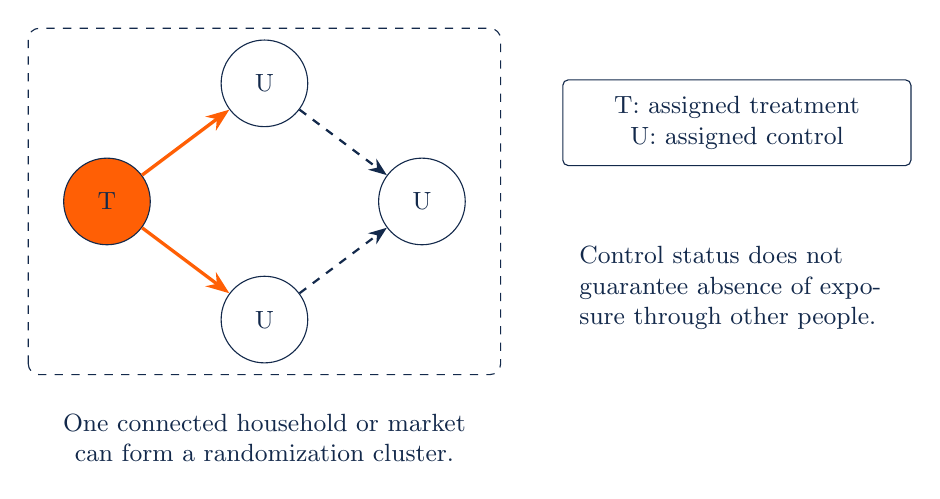
\begin{tikzpicture}[v/.style={circle,draw=IlliniBlue,minimum size=11mm},t/.style={v,fill=IlliniOrange}]
\node[t] (t) at (0,0) {T};\node[v] (a) at (2,1.5) {U};\node[v] (b) at (2,-1.5) {U};\node[v] (c) at (4,0) {U};
\draw[accent] (t)--(a);\draw[accent] (t)--(b);\draw[edge,dashed] (a)--(c);\draw[edge,dashed] (b)--(c);
\draw[IlliniBlue,dashed,rounded corners] (-1,-2.2) rectangle (5,2.2);
\node[align=center] at (2,-3) {One connected household or market\\can form a randomization cluster.};
\node[box,text width=4cm] at (8,1) {T: assigned treatment\\U: assigned control};
\node[align=left,text width=4cm] at (8,-1.1) {Control status does not guarantee absence of exposure through other people.};
\end{tikzpicture}

\end{adjustbox}
\endgroup
\par\medskip
{\small Synthetic store network with effects beyond assigned units.\par}
\note{The chain-wide outcome may change less than the treated-store outcome. Assignment and outcome aggregation should follow the managerial decision.

M6, Section 6.10, Marketing Analytics Lecture Notes. \url{../06_Lecture_Notes/modules/M06_Causal_Inference_and_Experiments.md}}
\end{frame}
\begin{frame}{Coding Exercise: Policy Value}
\usebeamercolor[fg]{normal text}
\vfill
\begin{slidebullets}
\item Reproduce raw rates and inverse-propensity values.
\item Check them using within-group averages.
\item Set one logging probability to zero and explain the missing comparison.
\end{slidebullets}
\vfill
\note{Run ../03\_Data\_and\_Code/Lecture\_Examples/session\_examples.py S10. A correct implementation flags unsupported target actions. Silently dropping the unsupported group changes the target population.

M6, Section 6.11, Marketing Analytics Lecture Notes. \url{../06_Lecture_Notes/modules/M06_Causal_Inference_and_Experiments.md}}
\end{frame}
\begin{frame}{Information and Exposure}
\usebeamercolor[fg]{normal text}
\vfill
\begin{slidebullets}
\item A recommendation can draw attention to an item.
\item A personalized endorsement can also change beliefs.
\item Separate interventions can identify these channels.
\end{slidebullets}
\vfill
\note{The MovieLens experiment discussed in the notes distinguishes recommendation and exposure-only conditions. The relevant outcome and information treatment should be stated before attributing a response to personalization.

M6, Section 6.10.1, Marketing Analytics Lecture Notes. \url{../06_Lecture_Notes/modules/M06_Causal_Inference_and_Experiments.md}}
\end{frame}
\begin{frame}{A Policy Value for Whom?}
\usebeamercolor[fg]{normal text}
\vfill
\begin{slidebullets}
\item Clicks and sales can rise while customer value falls.
\item A causal estimate concerns the outcome that was actually measured.
\item Record refusal, completion, and customer time when procedures change.
\end{slidebullets}
\vfill
\note{A valid causal effect on conversion does not identify the welfare effect without information about customer values and costs. The next measurement should address the missing part of the decision.

ETHICS\_AND\_REGULATION.md, M6.}
\end{frame}
\begin{frame}{Causal-Design Discussion}
\usebeamercolor[fg]{normal text}
\vfill
\begin{slidebullets}
\item What would the treated group have experienced without the policy?
\item Which group or action lacks comparable support?
\item What institutional evidence strengthens the proposed comparison?
\end{slidebullets}
\vfill
\note{A causal interpretation rests on the comparison and assumptions. A flexible estimator does not supply a missing assignment mechanism or recover outcomes outside support.

M6, Section 6.11, Marketing Analytics Lecture Notes. \url{../06_Lecture_Notes/modules/M06_Causal_Inference_and_Experiments.md}}
\end{frame}
\end{document}
